\chapter*{Exploratory Data Analysis}\label{chap:eda}
An extensive analysis of the data that will be used during the development process was carried out. This chapter presents the results of this analysis, which are used to guide the development of the system.


\section{MULTI-VP Dataset}\label{sec:data_prelim_analysis}
The data used by MULTI-VP and, consequently, the RNN prediction model consists of magnetogram data from the Wilcox Solar Observatory. Each file contains 12 columns representing measurements of the magnetic field in the solar atmosphere at different heights. Every variable comprises 640 points (abscissas) measured at different radial distances from the Sun (up to 30 Solar radii). In addition, the data is distributed evenly throughout five profiles, each consisting of solar wind measurements at different surface locations. For this work, only six columns will be used, as the others are derivations of these and, thus, are obtained with these columns. 

The data columns can be seen in Table \ref{tab:multivp_columns}. These are divided into two parts: the input and the output. The former comprises the set of variables used by the simulation to approximate solar wind conditions, and the latter the initial expert guesses needed to kickstart the multiple flux simulation. The input data includes the magnetic field amplitude, $B$, the flux tube inclination, $\alpha$, and the radial coordinate, $R$. The output data consists of the number of charged particles per unit volume, $n$, the velocity, $v$, and the temperature, $T$.

\begin{table}[ht]
    \caption{Data columns of magnetogram used by MULTI-VP.}
    \label{tab:multivp_columns}
    \begin{subtable}[h]{0.32\textwidth}
        \centering
        \begin{tabular}{lcc}
        \hline
        \multicolumn{3}{c}{Input (Partial Flows)}                              \\ \hline
        $R${[}$R_{sun}${]} & $B${[}$G${]} & $\alpha${[}$deg${]} \\ \hline
        \end{tabular}
    \end{subtable}
    \begin{subtable}[h]{0.32\textwidth}
        \centering
        \begin{tabular}{ccc}
        \hline
        \multicolumn{3}{c}{Output (Estimations)}                           \\ \hline
        $n${[}$cm^{-3}${]} & $v${[}$km/s${]} & $T${[}$MK${]} \\ \hline
        \end{tabular}
    \end{subtable}
\end{table}

A joint plot of the input variables can be seen in Fig. \ref{fig:jointplot_input}. From these plots, it can be concluded that several input files constitute anomalous data. This is clear from the graph of $B$, with files that significantly deviate from the rest. 


\begin{figure}[h]
    \centering
    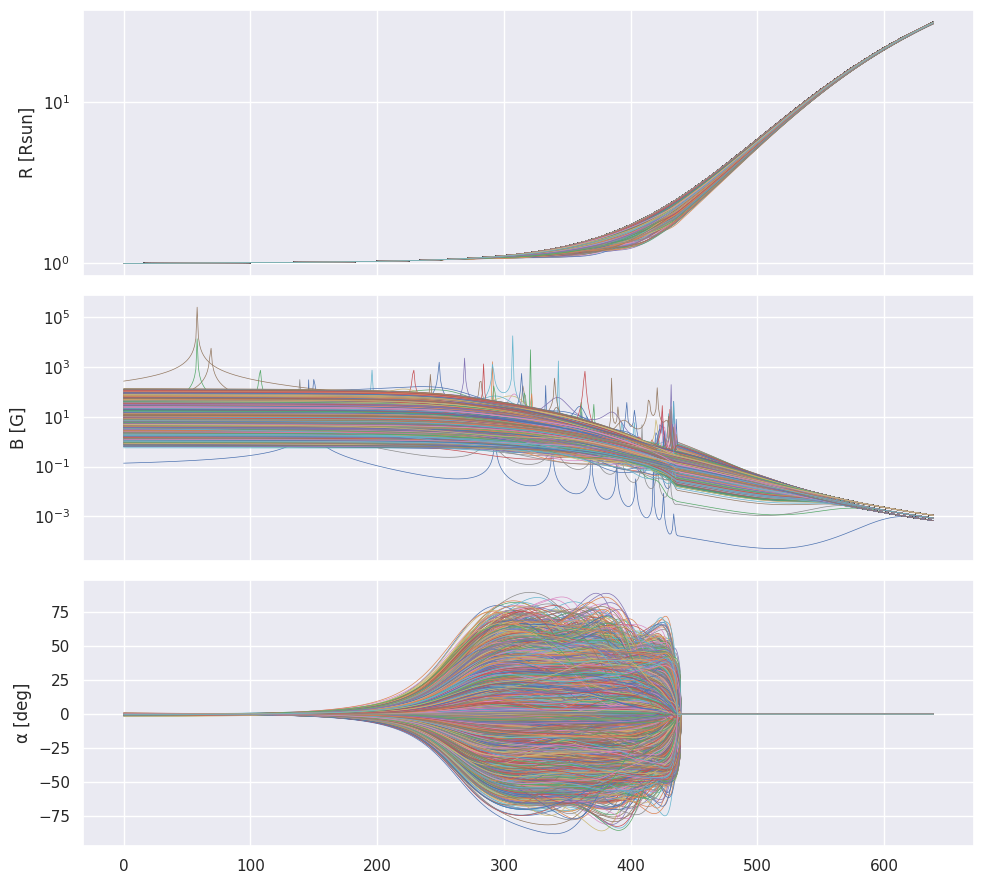
\includegraphics[width=0.8\textwidth]{figures/joint_input_cols.png}
    \caption{Joint plot of the input variables of each file used in this work. The first row is the plot of the radial coordinate radius, $R$, the second the magnetic field, $B$, and the last the flux tube inclination $\alpha$. All are plotted in function of position in the magnetogram file.}
    \label{fig:jointplot_input}
\end{figure}

% TODO refs para research statement
As previously explained, MULTI-VP requires initial expert guesses to kickstart the simulation. These guesses consist of the output variables presented in Table \ref{tab:multivp_columns} and, during the simulation, are approximated to better solutions. In line with the work carried out in \cite{barros_InitialConditionEstimation_}, we will be using the outputs of previous simulations as initial guesses (refer to chapter \ref{chap:research_proposal} for more details).


Fig. \ref{fig:jointplot_output} shows the joint plot of the output variables. Similar to the input plots, several faulty predictions can be seen in all variable plots, which are the result of simulations carried out on anomalous inputs.

\begin{figure}[h]
    \centering
    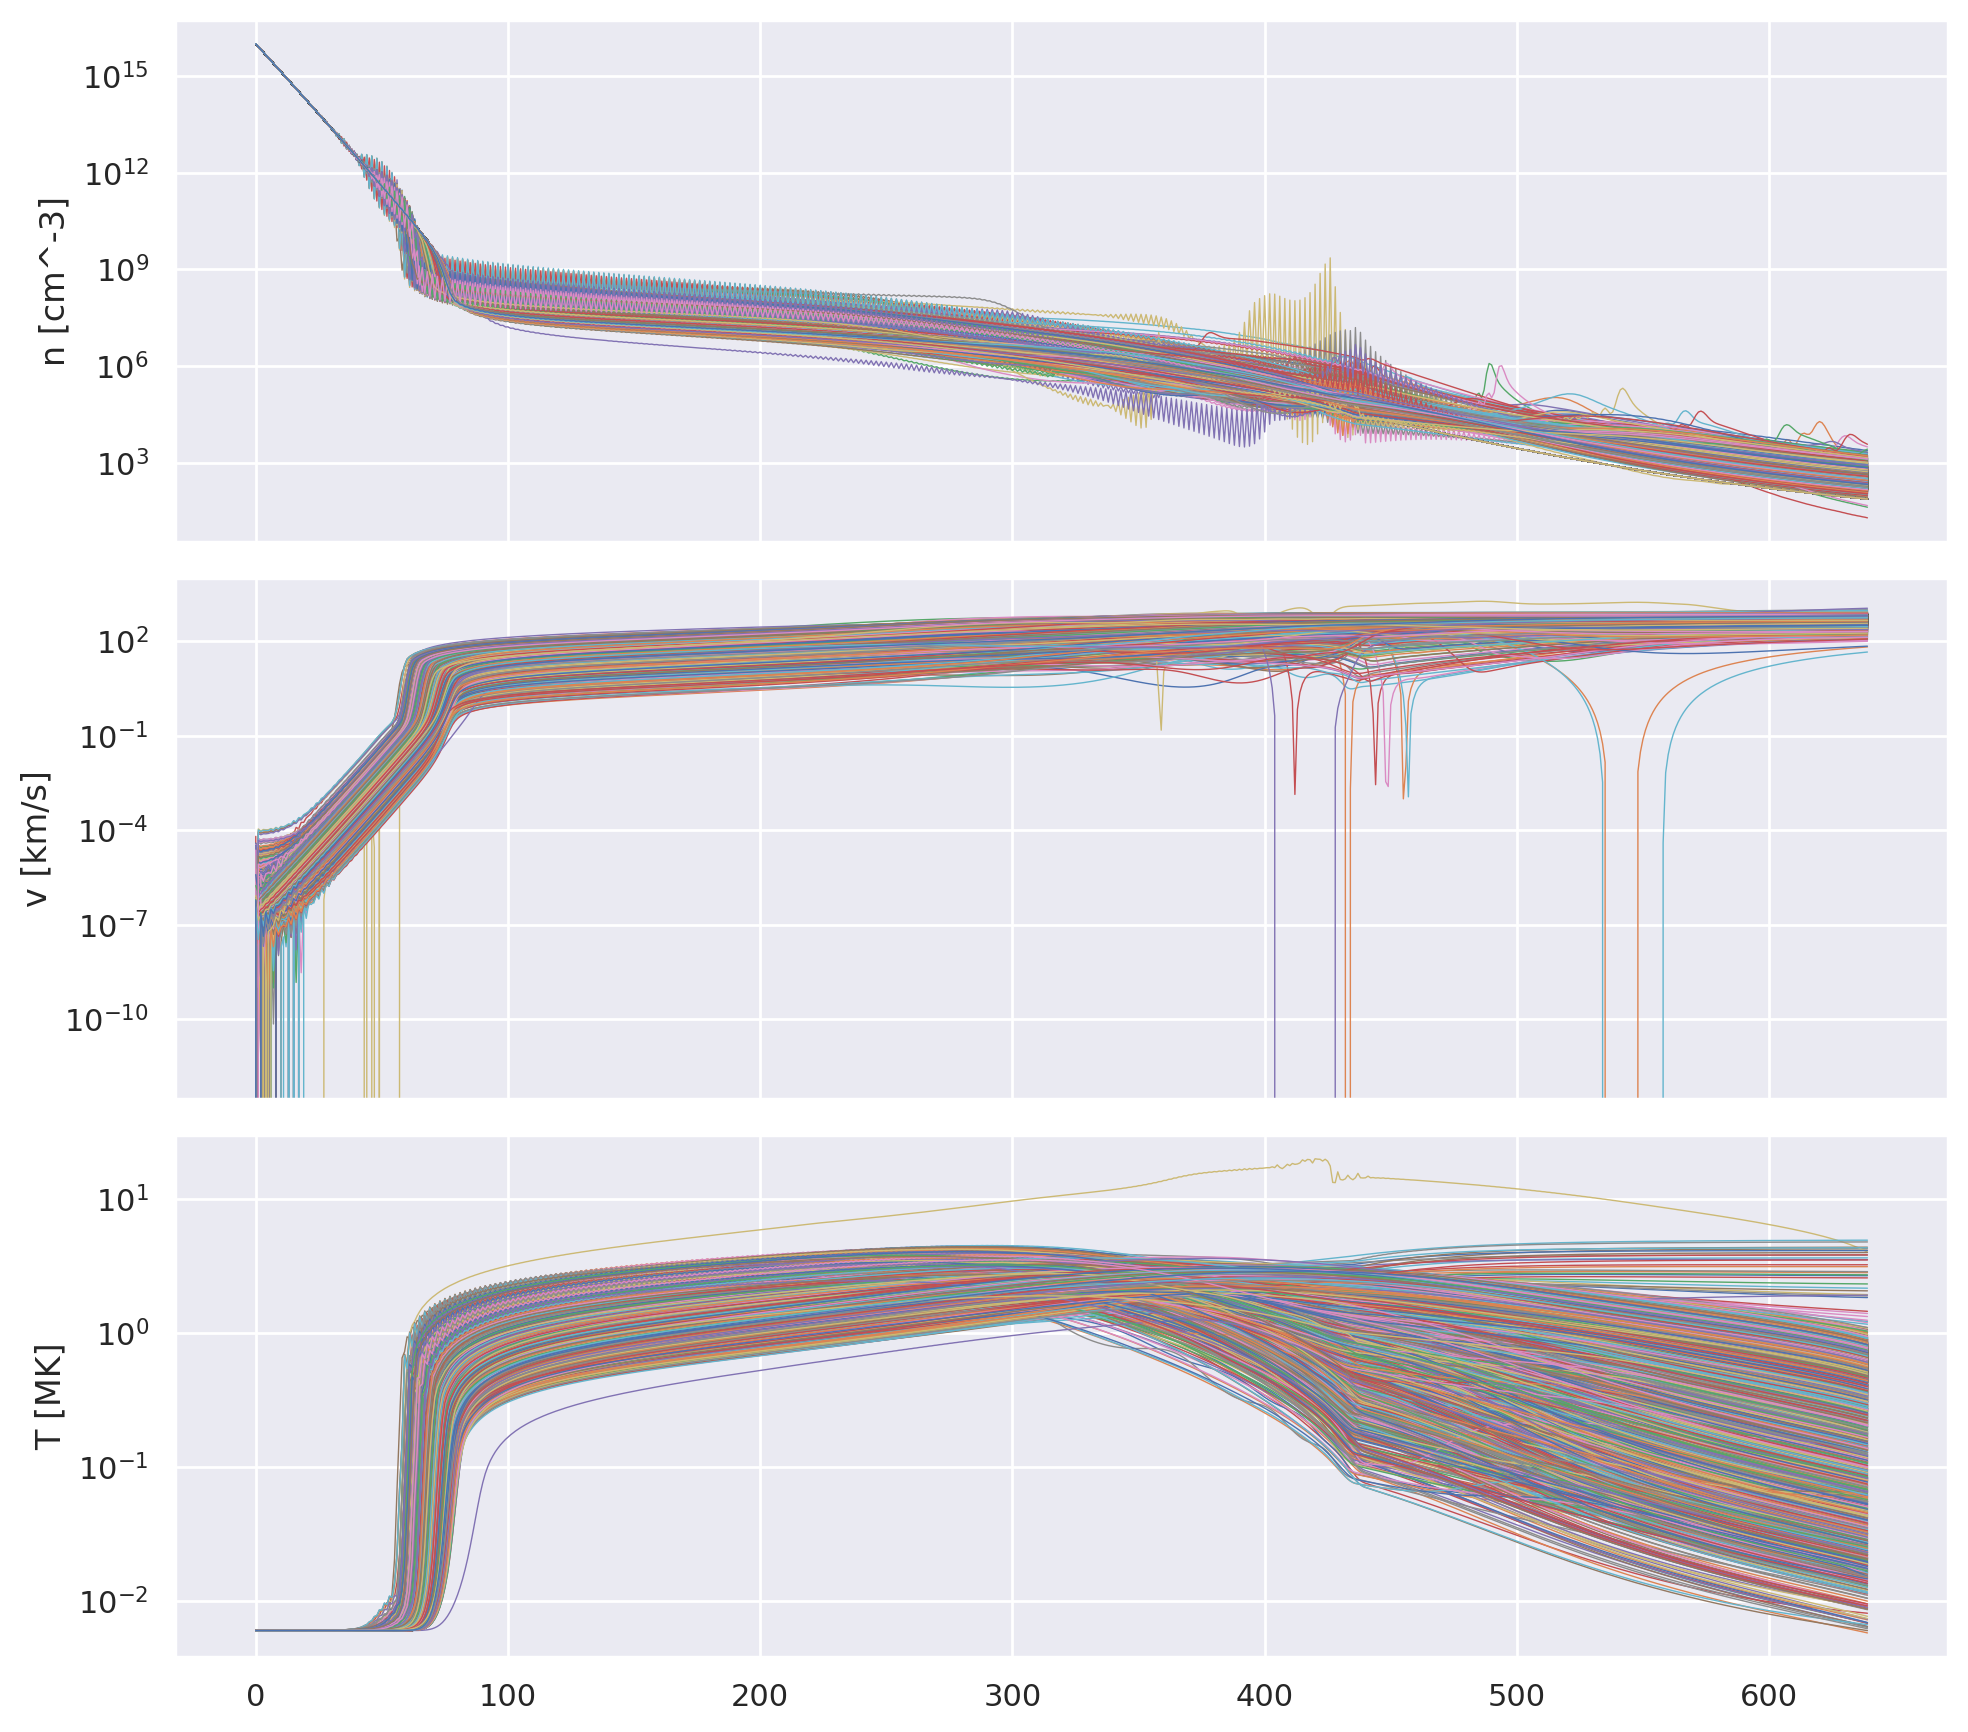
\includegraphics[width=0.8\textwidth]{figures/joint_output_cols.png}
    \caption{Joint plot of the output variables of each file used in this work. The first row is the plot of the number of charged particles per unit volume, $n$, the second the velocity, $v$, and the last the temperature, $T$. All are plotted in function of position in the magnetogram file.}
    \label{fig:jointplot_output}
\end{figure}

A preliminary statistical analysis of the data can be seen in tables \ref{tab:data_stats}. In it, the mean, standard deviation, minimum, maximum, and quartiles of each variable are presented.

Out of the three input columns used, the magnetic field ($B$) has the highest standard deviation, which might indicate that this column is more prone to anomalies than the others. The radial coordinate ($R$) has the lowest standard deviation, which is expected, as it is a constant value for each file. The output variables have a similar standard deviation, with the number of charged particles per unit volume ($n$) having the highest and the temperature ($T$) the lowest. The velocity ($v$) has a standard deviation similar to that of the temperature.

\begin{table}[]
    \caption{Statistical Analysis of the dataset.}
    \label{tab:data_stats}
    \begin{tabular}{@{}lrrrrrr@{}}
    \toprule
           & R {[}Rsun{]} & B {[}G{]} & $\alpha$ {[}deg{]} & $n${[}$cm^{-3}${]} & $v${[}$km/s${]} & $T${[}$MK${]} \\ \midrule
    mean   & 4.755        & 5.471     & 1.885              & 8.630e+13 & 2.553e+02  & 1.384     \\
    std    & 7.165        & 9.178e+01 & 1.472e+01          & 6.839e+14 & 2.148e+02  & 8.968e-01 \\
    min    & 1.000        & 5.122e-05 & -8.763e+01         & 1.973e+01 & -6.757e-03 & 5.765e-03 \\
    $25\%$ & 1.021        & 4.051e-02 & -1.079e-01         & 1.622e+04 & 4.926e+01  & 7.179e-01 \\
    $50\%$ & 1.151        & 2.095     & 0.000              & 2.351e+06 & 2.110e+02  & 1.337     \\
    $75\%$ & 4.250        & 5.582     & 9.997e-01          & 2.132e+07 & 4.508e+02  & 2.098     \\
    max    & 3.150e+01    & 2.470e+05 & 8.925e+01          & 1.010e+16 & 1.889e+03  & 1.990e+01 \\ \bottomrule
    \end{tabular}
    \end{table}


\begin{figure}[h]
    \centering
    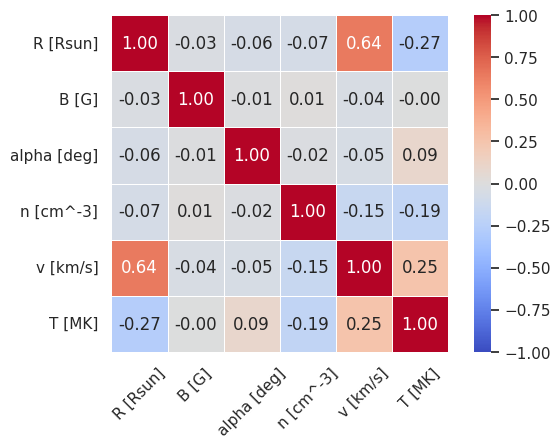
\includegraphics[width=0.8\textwidth]{figures/variables_corrplot.png}
    \caption{Correlation plot of all variables used in this work.}
    \label{fig:corrplot}
\end{figure}

In addition to these statistics, the correlation between the variables can be seen in Fig. \ref{fig:corrplot}. There is virtually no correlation between the input variables ($R$, $B$, and $\alpha$), which is expected, as they are independent of each other. 

% TODO prof check this
The output variables ($n$, $v$, and $T$) are somewhat correlated. The temperature, $T$, is positively correlated with the velocity of the solar wind, $v$, which is expected as with higher wind speeds the particles there is a tendency for higher temperatures. The opposite is true for the volume density of the solar wind, $n$, which is negatively correlated with the temperature. This is expected as with higher densities, the particles will have less kinetic energy and, therefore, a lower temperature. The velocity of the solar wind is also slightly negatively correlated with the volume density.

A high correlation between the radial coordinate $R$ and the velocity $v$ can be observed, as the velocity is expected to increase with distance from the Sun. Additionally, the temperature of the solar wind drops as the distance to the Sun increases, which is reflected in the negative correlation between $R$ and $T$.

\begin{figure}
    \centering
    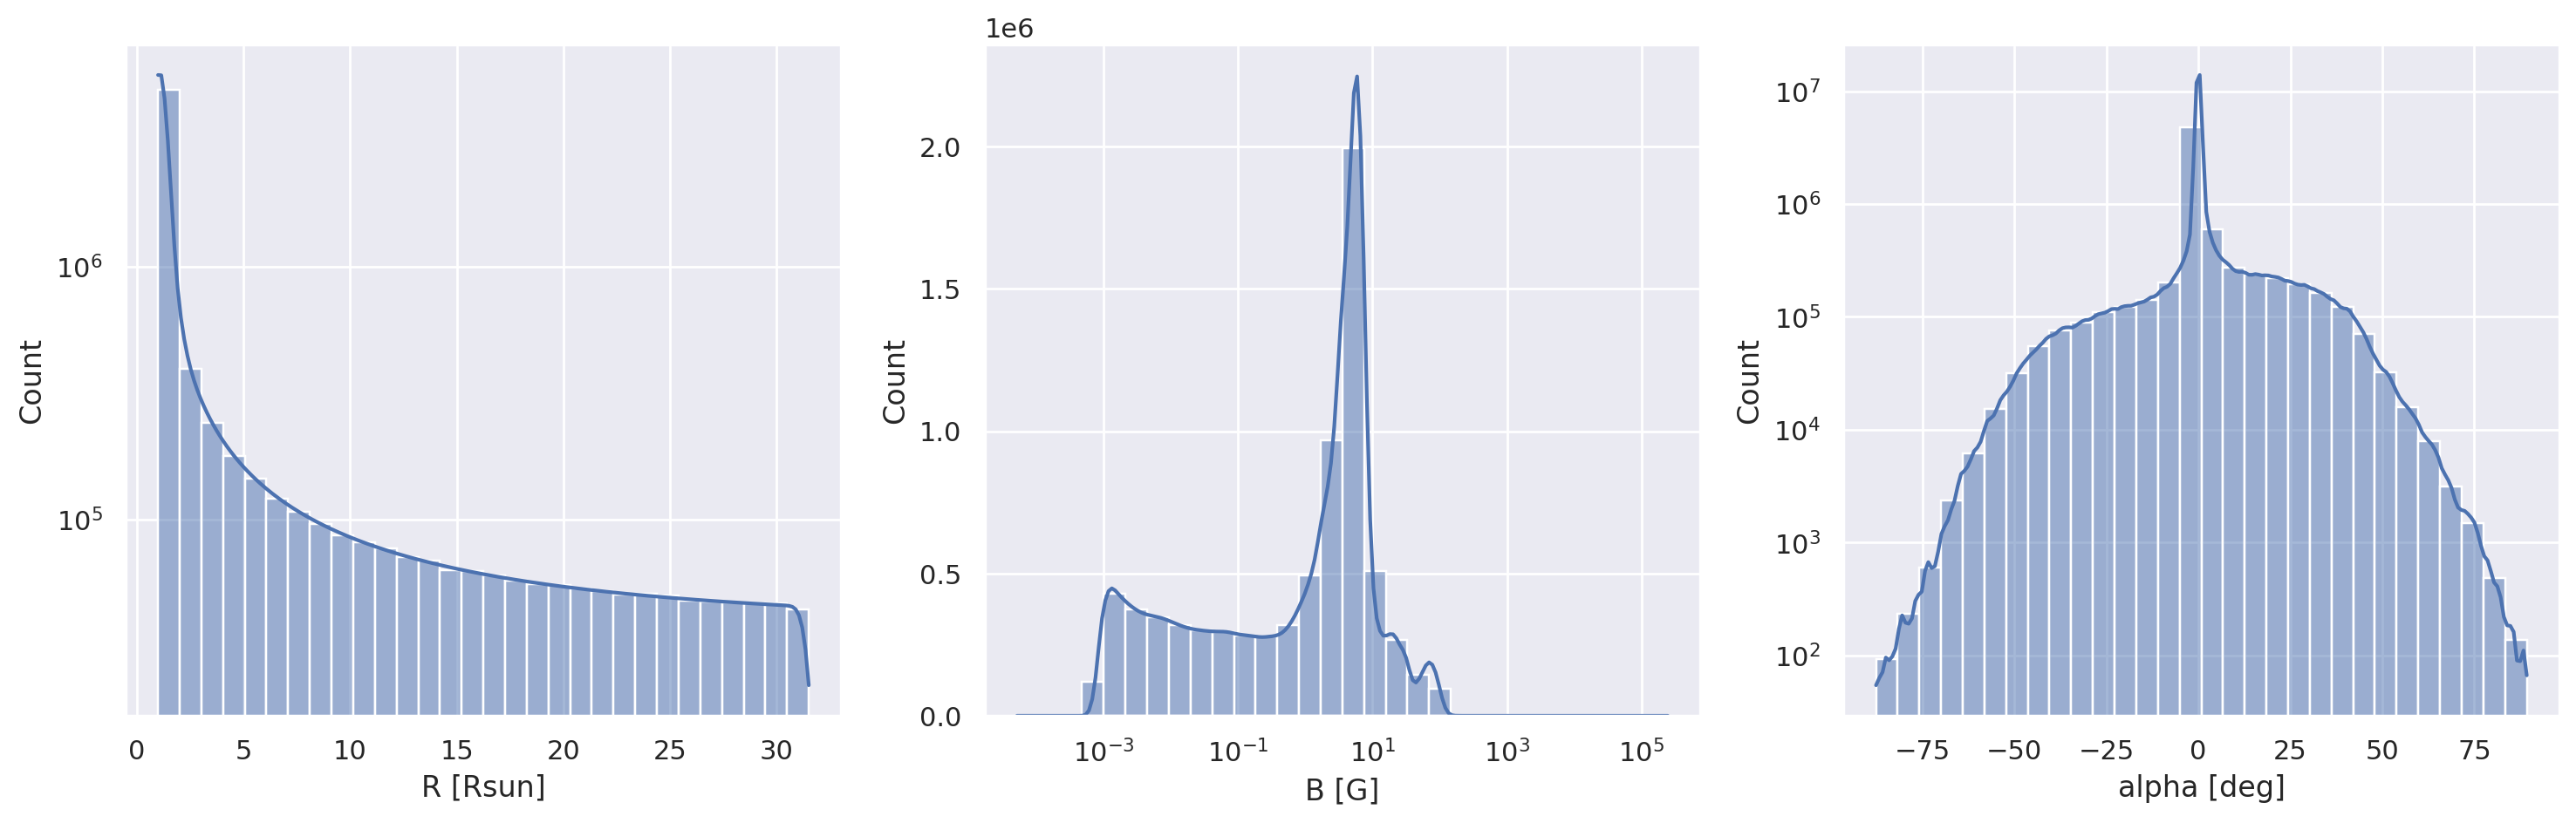
\includegraphics[width=\textwidth]{figures/input_vars_distribution.png}
    \caption{Distribution of the input variables}
    \label{fig:input_vars_distr}
\end{figure}

A distribution plot of each of the input variables can be seen in Fig. \ref{fig:input_vars_distr}. The values of the radial coordinate $R$ range from 1 to about 31.5 as was already seen by looking at Table \ref{tab:data_stats}, with most values being concentrated around 1. % TODO

